\documentclass{beamer}


% Beamer settings
\usecolortheme{rose}
\beamertemplatenavigationsymbolsempty
\setbeamertemplate{footline}[frame number]

\titlegraphic{%

\includegraphics[height=1cm]{logo-full-colour.png}}

\addtobeamertemplate{frametitle}{}{%
\begin{tikzpicture}[remember picture,overlay]
\node[anchor=north east,yshift=2pt] at (current page.north east) {
\includegraphics[height=1cm]{logo-full-colour.png}};
\end{tikzpicture}}

% Packages
\usepackage{amsmath}

\usepackage{tikz}
\usetikzlibrary{positioning}
\usetikzlibrary{fit}

\usepackage{pgfplots}
\usepgfplotslibrary{fillbetween}

\usepackage{minted}
\usepackage[T1]{fontenc} % Required by minted to ensure dollar signs are produced instead of pound (sterling) signs

\usepackage{multicol}

\usepackage{booktabs}

\usepackage{adjustbox}

% Author
\author{Simon McIntosh-Smith \& Tom Deakin\\University of Bristol}

\date{}



\title{OpenMP for Computational Scientists}
\subtitle{3: Vectoristation and optimisations}

\begin{document}

\frame{\titlepage}

%-------------------------------------------------------------------------------
\begin{frame}
\frametitle{Outline}
Now you know how to parallelise programs using OpenMP, how do you write fast programs in OpenMP?
\begin{itemize}
  \item Performance analysis
  \item Vectorisation
  \item The cache hierarchy
  \item Memory access patterns
\end{itemize}
\end{frame}

%-------------------------------------------------------------------------------
\begin{frame}
\frametitle{Roofline models}
\end{frame}

%-------------------------------------------------------------------------------
\begin{frame}
\frametitle{Vectorisation}
$$C=A+B$$
\begin{columns}
\begin{column}{0.5\textwidth}
Scalar operations \\
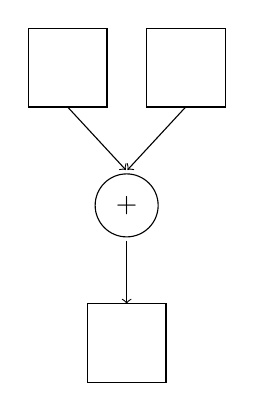
\begin{tikzpicture}
  \draw (-0.5,2) rectangle (0.5,3);
  \draw (1,2) rectangle (2,3);
  \draw[->] (0,2) -- (.74,1.2);
  \draw[->] (1.5,2) -- (.76,1.2);
  \draw (.75,.75) circle (.4cm);
  \draw (.75,.75) node {$+$};
  \draw[->] (.75,0.3) -- (.75,-0.5);
  \draw (.25,-1.5) rectangle (1.25,-0.5);
\end{tikzpicture}
\end{column}

\begin{column}{0.5\textwidth}
Vector operations \\
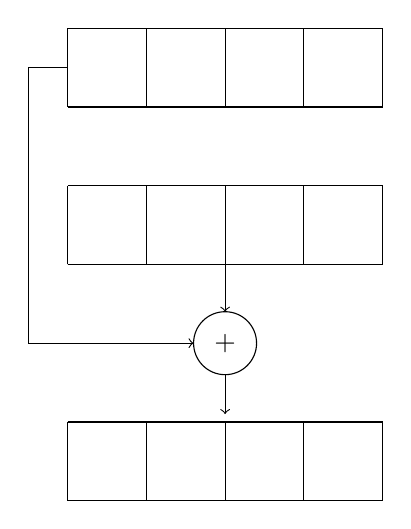
\begin{tikzpicture}
  \draw[step=1cm] (0,2) grid (4,3);
  \draw[step=1cm] (0,0) grid (4,1);
  \draw[->] (2,0) -- (2,-0.6);
  \draw[->] (0,2.5) -- (-0.5,2.5) -- (-0.5,-1) -- (1.6,-1);
  \draw (2,-1) circle (.4cm);
  \draw (2,-1) node {$+$};
  \draw[->] (2,-1.4) -- (2,-1.9);
  \draw[step=1cm] (0,-3) grid (4,-2);
\end{tikzpicture}
\end{column}
\end{columns}

\end{frame}

%-------------------------------------------------------------------------------
\begin{frame}
\frametitle{Why vectorise?}

\end{frame}

%-------------------------------------------------------------------------------
\begin{frame}
\frametitle{Auto-vectorisation}
Compiler reports
\end{frame}

%-------------------------------------------------------------------------------
\begin{frame}
\frametitle{OpenMP SIMD}
\end{frame}

%-------------------------------------------------------------------------------
\begin{frame}
\frametitle{Derived types}
AoS vs SoA
\end{frame}

%-------------------------------------------------------------------------------
\begin{frame}
\frametitle{Alignment}
Align and tell compiler
Issues with 2D
\end{frame}

%-------------------------------------------------------------------------------
\begin{frame}
\frametitle{Cache hierarchy}
\end{frame}

%-------------------------------------------------------------------------------
\begin{frame}
\frametitle{Memory access patterns}
\end{frame}

%-------------------------------------------------------------------------------
\section{Exercise}
\begin{frame}
\frametitle{Exercise}
\begin{itemize}
  \item Take your parallel 5-point stencil code and optimise.
  \item Think about:
    \begin{itemize}
      \item Memory access patterns
      \item Vectorisation
    \end{itemize}
  \item Note down the performance differences your optimisations make.
\end{itemize}
\end{frame}

%-------------------------------------------------------------------------------

\end{document}
